\documentclass{sig}

\usepackage{algorithm}
\usepackage{algpseudocode}
\usepackage{amsmath}
\usepackage{appendix}
\usepackage{balance}
\usepackage{caption}
\usepackage{color}
\usepackage{comment}
\usepackage{epstopdf}
\usepackage{graphicx}
\usepackage{listings}
\usepackage{mathtools}
\usepackage{microtype}
\usepackage{multirow}
\usepackage{pdfpages}
\usepackage{subcaption}
\usepackage{subfig}
\usepackage{tabularx}
\usepackage{times}
\usepackage{url}
\usepackage{xcolor}
\usepackage{xspace}
\usepackage{bm}
\usepackage{mdwlist}

\newcommand{\subparagraph}{}
\usepackage{titlesec}

%\titlespacing{\section}{0ex}{0.8ex}{0ex}
%\titlespacing{\subsection}{0ex}{0.8ex}{0ex}
%\titlespacing{\subsubsection}{0ex}{0.7ex}{0ex}
%\setlength{\parskip}{0ex}

\algrenewcommand\alglinenumber[1]{\scriptsize #1:}

\makeatletter
\renewcommand*{\ALG@name}{Investing Rule}
\makeatother


\usepackage{breqn}
\interfootnotelinepenalty=10000

\newcommand{\todo}[1]{\textcolor{blue}{TODO: #1}}
\newcommand{\done}[1]{\textcolor{green}{DONE#1}}
\newcommand{\tim}[1]{\textcolor{red}{Tim: #1}}
\newcommand{\lore}[1]{\textcolor{blue}{Lorenzo: #1}}
\newcommand{\ez}[1]{\textcolor{orange}{ez: #1}}
\newcommand{\sam}[1]{\textcolor{purple}{sam: #1}}
\newcommand{\carsten}[1]{\textcolor{brown}{Carsten: #1}}

\newcommand{\naive}{na\"{\i}ve\xspace}
\newcommand{\Naive}{Na\"{\i}ve\xspace}
\newcommand{\naively}{na\"{\i}vely\xspace}

\newcommand{\ainv}{$\alpha$-investing }
\newcommand{\sfdr}{Sequential-FDR }
\newcommand{\mfdre}{$mFDR_{\eta}$ }
\newcommand{\mfdr}[1]{$mFDR_{#1}$}
\newcommand{\Ex}[1]{E\left[#1\right]}
\newcommand{\Prob}[1]{\text{P}\left(#1\right)}
\newcommand{\CProb}[2]{\text{P}\left(#1|#2\right)}
\newcommand{\pval}{$p$-value }
\newcommand{\pvals}{$p$-values }


\newcommand{\system}{{\sc Aware}}
\newcommand{\Chi}{\mathcal{X}}

\newtheorem{theorem}{Theorem}
\newtheorem{lemma}{Lemma}


%\setlength\abovedisplayskip{0pt plus 2pt minus 0pt}
%\setlength\belowdisplayskip{0pt plus 2pt minus 0pt}

%\makeatletter
%\g@addto@macro \normalsize {%
%\setlength\abovedisplayskip{0pt plus 2pt minus 0pt}%
%\setlength\belowdisplayskip{0pt plus 2pt minus 0pt}%
%\setlength\abovedisplayshortskip{0pt plus 2pt minus 0pt}%
%\setlength\belowdisplayshortskip{0pt plus 2pt minus 0pt}%
%}
%\makeatother

%\makeatletter
%\g@addto@macro \small {%
%\setlength\abovedisplayskip{0pt plus 2pt minus 0pt}%
%\setlength\belowdisplayskip{2pt plus 2pt minus 0pt}%
%\setlength\abovedisplayshortskip{0pt plus 2pt minus 0pt}%
%\setlength\belowdisplayshortskip{2pt plus 2pt minus 0pt}%
%}
%\makeatother

\DeclareMathOperator*{\argmin}{\arg \min}
\DeclarePairedDelimiter\ceil{\lceil}{\rceil}

\captionsetup{font={bf}}

%\newcommand{\system}{{\sc Vizdom}}

\newcommand{\specialcell}[2][c]{
  \begin{tabular}[#1]{@{}c@{}}#2\end{tabular}}

\definecolor{dark-gray}{gray}{0.2}

\newenvironment{packed_item}{
\begin{list}{$\bullet$}{
  \setlength{\itemsep}{-2pt}
  \setlength{\parskip}{1pt}
  \setlength{\labelwidth}{15 pt}
  \setlength{\leftmargin}{10pt}
  \setlength{\itemindent}{0pt}}
}{\end{list}}

% for floated 2 column equations
\newcounter{tempEquationCounter}
\newcounter{thisEquationNumber}
\newenvironment{floatEq}
{\setcounter{thisEquationNumber}{\value{equation}}\addtocounter{equation}{1}% record equation as happened and remember number
\begin{figure*}[t]% float following equation across columns
\normalsize\setcounter{tempEquationCounter}{\value{equation}}% record current equation number in floated location
\setcounter{equation}{\value{thisEquationNumber}}% use previous equation number
}
{\setcounter{equation}{\value{tempEquationCounter}}% set back to equation number in floated location
\hrulefill\vspace*{4pt}% add a horizontal rule separator
\end{figure*}% end float environment
}
\newtheorem{defi}{Definition}
\makeatletter
\newenvironment{subheuristic}[1]{%
  \def\subtheoremcounter{#1}%
  \refstepcounter{#1}%
  \protected@edef\theparentnumber{\csname the#1\endcsname}%
  \setcounter{parentnumber}{\value{#1}}%
  \setcounter{#1}{0}%
  \expandafter\def\csname the#1\endcsname{\theparentnumber\alph{#1}}%
  \ignorespaces
}{%
  \setcounter{\subtheoremcounter}{\value{parentnumber}}%
  \ignorespacesafterend
}
\makeatother
\newcounter{parentnumber}

\newtheorem{heuristic}{Heuristic}

\begin{document}



\title{Aware: Visual Data Exploration that Controls False Discoveries}

\numberofauthors{1}
\author{
\alignauthor
%\vspace*{-30pt}
%Paper \#178
\begin{tabular}{cccc}
\end{tabular}\\
%\vspace{1.5mm}
\affaddr{Department of Computer Science, Brown University}\\
%\vspace{0.75mm}
\{firstname\_lastname\}@brown.edu
%\email{\{firstname\_lastname\}@brown.edu}
}

%\numberofauthors{6}
%\author{
%\small{Andrew Crotty, Alex Galakatos, Kayhan Dursun, Tim Kraska, Ugur Cetintemel, Stan Zdonik} \\
%\small{Department of Computer Science, Brown University} \\
%\small{\{crottyan, agg, kayhan, kraskat, ugur, sbz\}@cs.brown.edu}
%}
\date{}
\maketitle

\begin{abstract}
Exploring data via visualization has become a popular way to understand complex data. Observations on the visual results are inherently hypotheses.  However, visually significant information may not carry any statistical significance. Moreover, visual data exploration produces observations dynamically and results in increasing numbers of false discoveries.  We present our solution based on Vizdom~\cite{vizdom}, namely, \system{}, a visual data exploration system that interacts with user to formulate visualization-based hypotheses and provides interactive control of false discoveries based on the recent advance in the subject~\cite{controlling-false-discoveries}.
\end{abstract}



\section{Introduction}
\label{sec:intro}
In the era of Big Data, interactive data exploration tools arise as an important mean to explore and derive insights from data through visualization.  
However, perceived interesting patterns in visual data representations, such as relationships or trends, may emerge from irrelevant random effects inherent to the data, such as random noises, large variances, insufficient samples, and biases. 
Without proper statistical control, users may mistake a distinct or dominant visual observation as statistically significant.  
On the other hand, systems that search and recommend visualizations automatically based on such interesting visual features further increase the chance of bogus insights.  
A recent study highlights these issues and shows that visualization and recommendation systems that do not consider the risk of false discovery, such as Vizdom~\cite{vizdom}, SeeDB~\cite{seedb} and Data Polygamy~\cite{polygamy}, become difficult to derive insights safely on real-world datasets \cite{binnig2017sustainable}.

False discovery due to random noise is pervasive in visual data exploration on real-world datasets. For example, when using Vizdom~\cite{vizdom} to explore a recently conducted survey on personal habits and opinions~\cite{binnig2017sustainable}, we observed that the preference on watching films on DVD produced visually different proportions of belief in aliens, as shown in Figure~\ref{fig:example} (A and B).
Just by visually examining these charts, users often falsely assumed that people who prefer to watch movies on DVD are more prone to believe in aliens even though this effect is not statistically significant.
%But such predictor proved neither much sensible nor statistically significant.  

Such observation-based hypotheses may be accumulated quickly as the user continues to explore a dataset, and hence dramatically raises the risk of spurious findings. 
With the same survey dataset, after searching through a few different comparisons we stumbled upon a visualization that suggests hair color predicts whether one knows about Michael Stonebraker, and it would be statistically significant if considered as a lone hypothesis. This phenomenon is often referred to as data dredging or $p$-hacking~\cite{head2015extent}, and formally known as the multiple comparison problem~\cite{shaffer1995multiple}.

Several challenges exist to control false insights in such interactive data exploration.  
The first question is what could even be considered as a hypothesis in visual data exploration.
In some cases users might explicitly specify certain hypotheses, but in other instances they do not formulate any hypothesis but still use visualization to infer about the data or to extract an insight.
An ideal system should assist users in hypothesis formulation and corresponding hypothesis test selection.

Second, interactive data exploration mandates that hypotheses are formulated dynamically based on the process of human decision making.  
However the classical statistical procedures such as Bonferroni~\cite{bonferroni1936teoria} and Sequential FDR~\cite{g2016sequential} are not dynamic as they require collecting all the hypotheses a priori before finalizing any significance result.  
Moreover these traditional techniques assume complete pass of the dataset, and thus would make the system non-interactive on larger data.  
Thus an ideal system for interactive control of false discovery should follow progressive computation, which proves to be a more appealing paradigm~\cite{vizdom, onlineagg, zgraggen2016progressive}.  

Finally, parts of the data exploration process can be automated through algorithmic search and recommendation. Such automatic data exploration should also be subject to false discovery control.  

In this demo, we present \system{}\footnote{\system{} stands for Quantifying the Uncertainty in Data Exploration.}, a first ``safe'' visual data exploration tool that addresses these challenges. 
In \system{}, we implemented recent techniques in interactive false discovery control that are both dynamic and progressive~\cite{zhao2016controlling}, apply them to visual data exploration and visualization recommendation, and expose them through a pen- \& touch-based user interface that simplifies and in some cases even automates the creation of hypothesis tests.


%Thus, to address theses challenges, we implemented the recent advance in interactive false discovery control that is both dynamic and progressive, and applied to both visual data exploration and recommendation~\cite{zhao2016controlling}. 

\begin{figure}
\centering
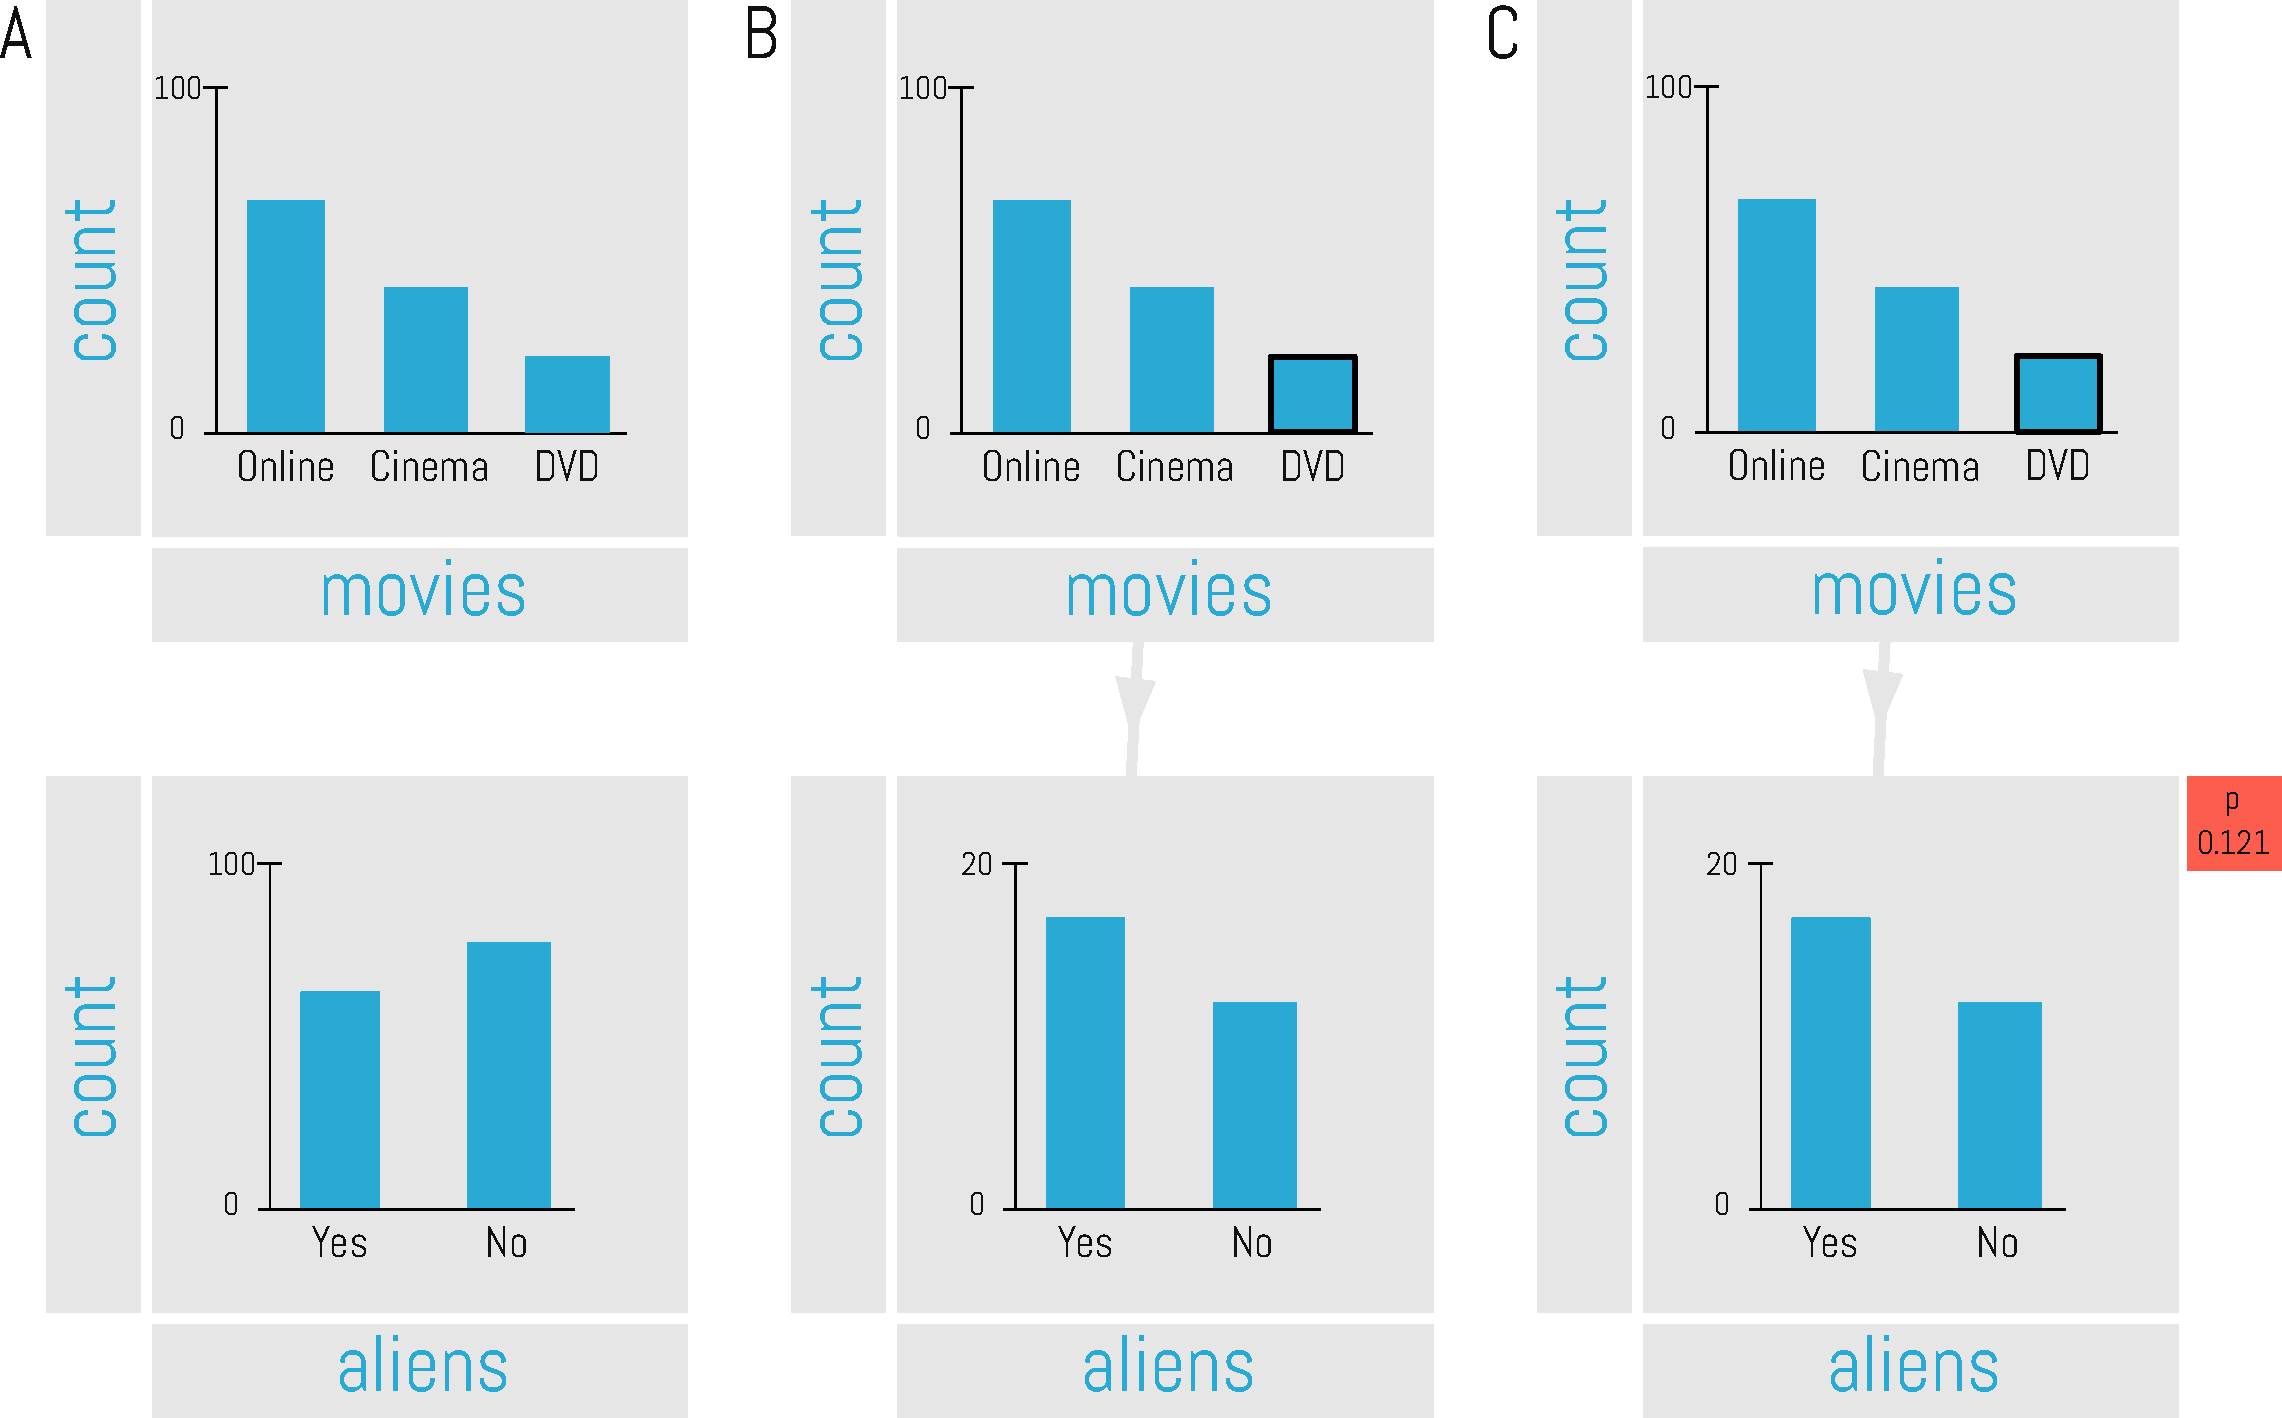
\includegraphics[width=0.47\textwidth]{figures/example}
\caption{Example of a visualization network where users might be led to false discoveries without automatic hypothesis formulation. (A) two separate visualizations showing preferences for watching movies and how many people believe in alien existence; (B) the two visualizations combined where the bottom one shows proportions of belief in alien existence for only people who like to watch movies on DVD, displaying a noticeable difference compared to the overall population. (C) same visualizations as before but now with automatic hypothesis formulation turned on, highlighting that the observed effect is not statistically significant.}
\label{fig:example}
\vspace{-3.5ex}
\end{figure}

\section{System Design}
\label{sec:system-design}

\subsection{User Interface}
\label{sec:ui}

\begin{comment}
As argued in the previous section, user feedback is essential in determining, tracking and controlling the right hypothesis during the data exploration process.
With \system~we created a system that applies our heuristic automatically to all visualizations. We designed \system~'s user interface with a few goals in mind.

First, the user should be able to see the hypotheses the system assumed so far, their \pvals, effect sizes and if they are considered significant and should be able to change, add or delete hypotheses at any given stage of the exploration. 

Second, hypotheses rejection decisions should never change based on future user actions unless the user explicitly asks for it. We therefore require an incremental procedure to control the multiple hypothesis risk that does not change its rejection decisions even if more hypothesis tests are executed.
For example, the system should not state that their is a significant age difference for not married highly educated people, and then later on revoke its assessment just because the user did more tests. 
More formally, if the system determined which hypotheses $m_1 ...  m_n$ are significant (i.e., it rejects the null) or not and the user changes the last hypothesis or adds an hypothesis $m_{n+1}$, which should be the most common cases, the significance of hypotheses $m_1..m_{n}$ should not change. 
However, if the user might change, delete, or add hypothesis $k \in {1,..,n}$, depending on the used procedure we might allow that the significance of hypotheses $m_{k+1}$ to $m_n$ might have to change as well.
%Furthermore, the system automatically reports on the {\bf effect size} as a color coded value based on Cohen's suggestions \cite{something}.
%This is according to best practice, as the effect size (e.g., the age difference) determines how big the observed difference is compared to the variance. 

Third, individual hypothesis descriptions should be augmented with information about how much data $n^{H1}$ the user has to add, under the assumption that the new data will follow the current observed distribution of the data, to make an hypothesis significant. 
While sounding counter-intuitive, as one might (wrongly) imply, it is possible to make any hypothesis true by adding more data, calculating this value is in some fields already common practice. 
For example, in genetics scientist often search (automatically) for correlations between genes and high-level effects (like cancer). 
If such a correlation is found, often because of the multiple hypothesis error the chance of a true discovery is tiny (i.e., the \pval is too high). 
In that case the scientist works backwards and estimates how much more genes she has to to sequence in order to make the hypothesis relevant, expecting that the new data (e.g., gene sequences) follow the same distribution of the data the scientist already has.
However, if the effect was just produced by chance, the new data will be more similar to the distribution of the null-hypothesis and the null will not be rejected.  
%Similar, it is possible for a rejected null-hypothesis to calculate how much data $n^{H0}$ has to be added if the null-hypothesis is true, until the null-hypothesis will be accepted. 
% Eli: This has no statistical meaning.
The required value is generally easy to calculate or approximate,  and are highly valuable for the end-user. 
A small value for $n^{H1}$ in relation to the number of totally tested hypotheses might be an indication that the power (i.e., the chance to accept a true alternative hypothesis) of the test was not sufficiently large. 

And finally, users should be able to bookmark important hypotheses. 
Our system uses default hypothesis throughout the exploration and the user might find it too cumbersome to correct everyone for his real intentions, there might be more hypotheses generated than the user intended to test. 
Even if all hypotheses are what the user was considering, some of them might be more important to her than others; the hypotheses the user would like to include in a presentation or show to her boss. 
A key key question becomes, what is the expected number of false discoveries among those important discoveries?
\end{comment}

\begin{figure}
\centering
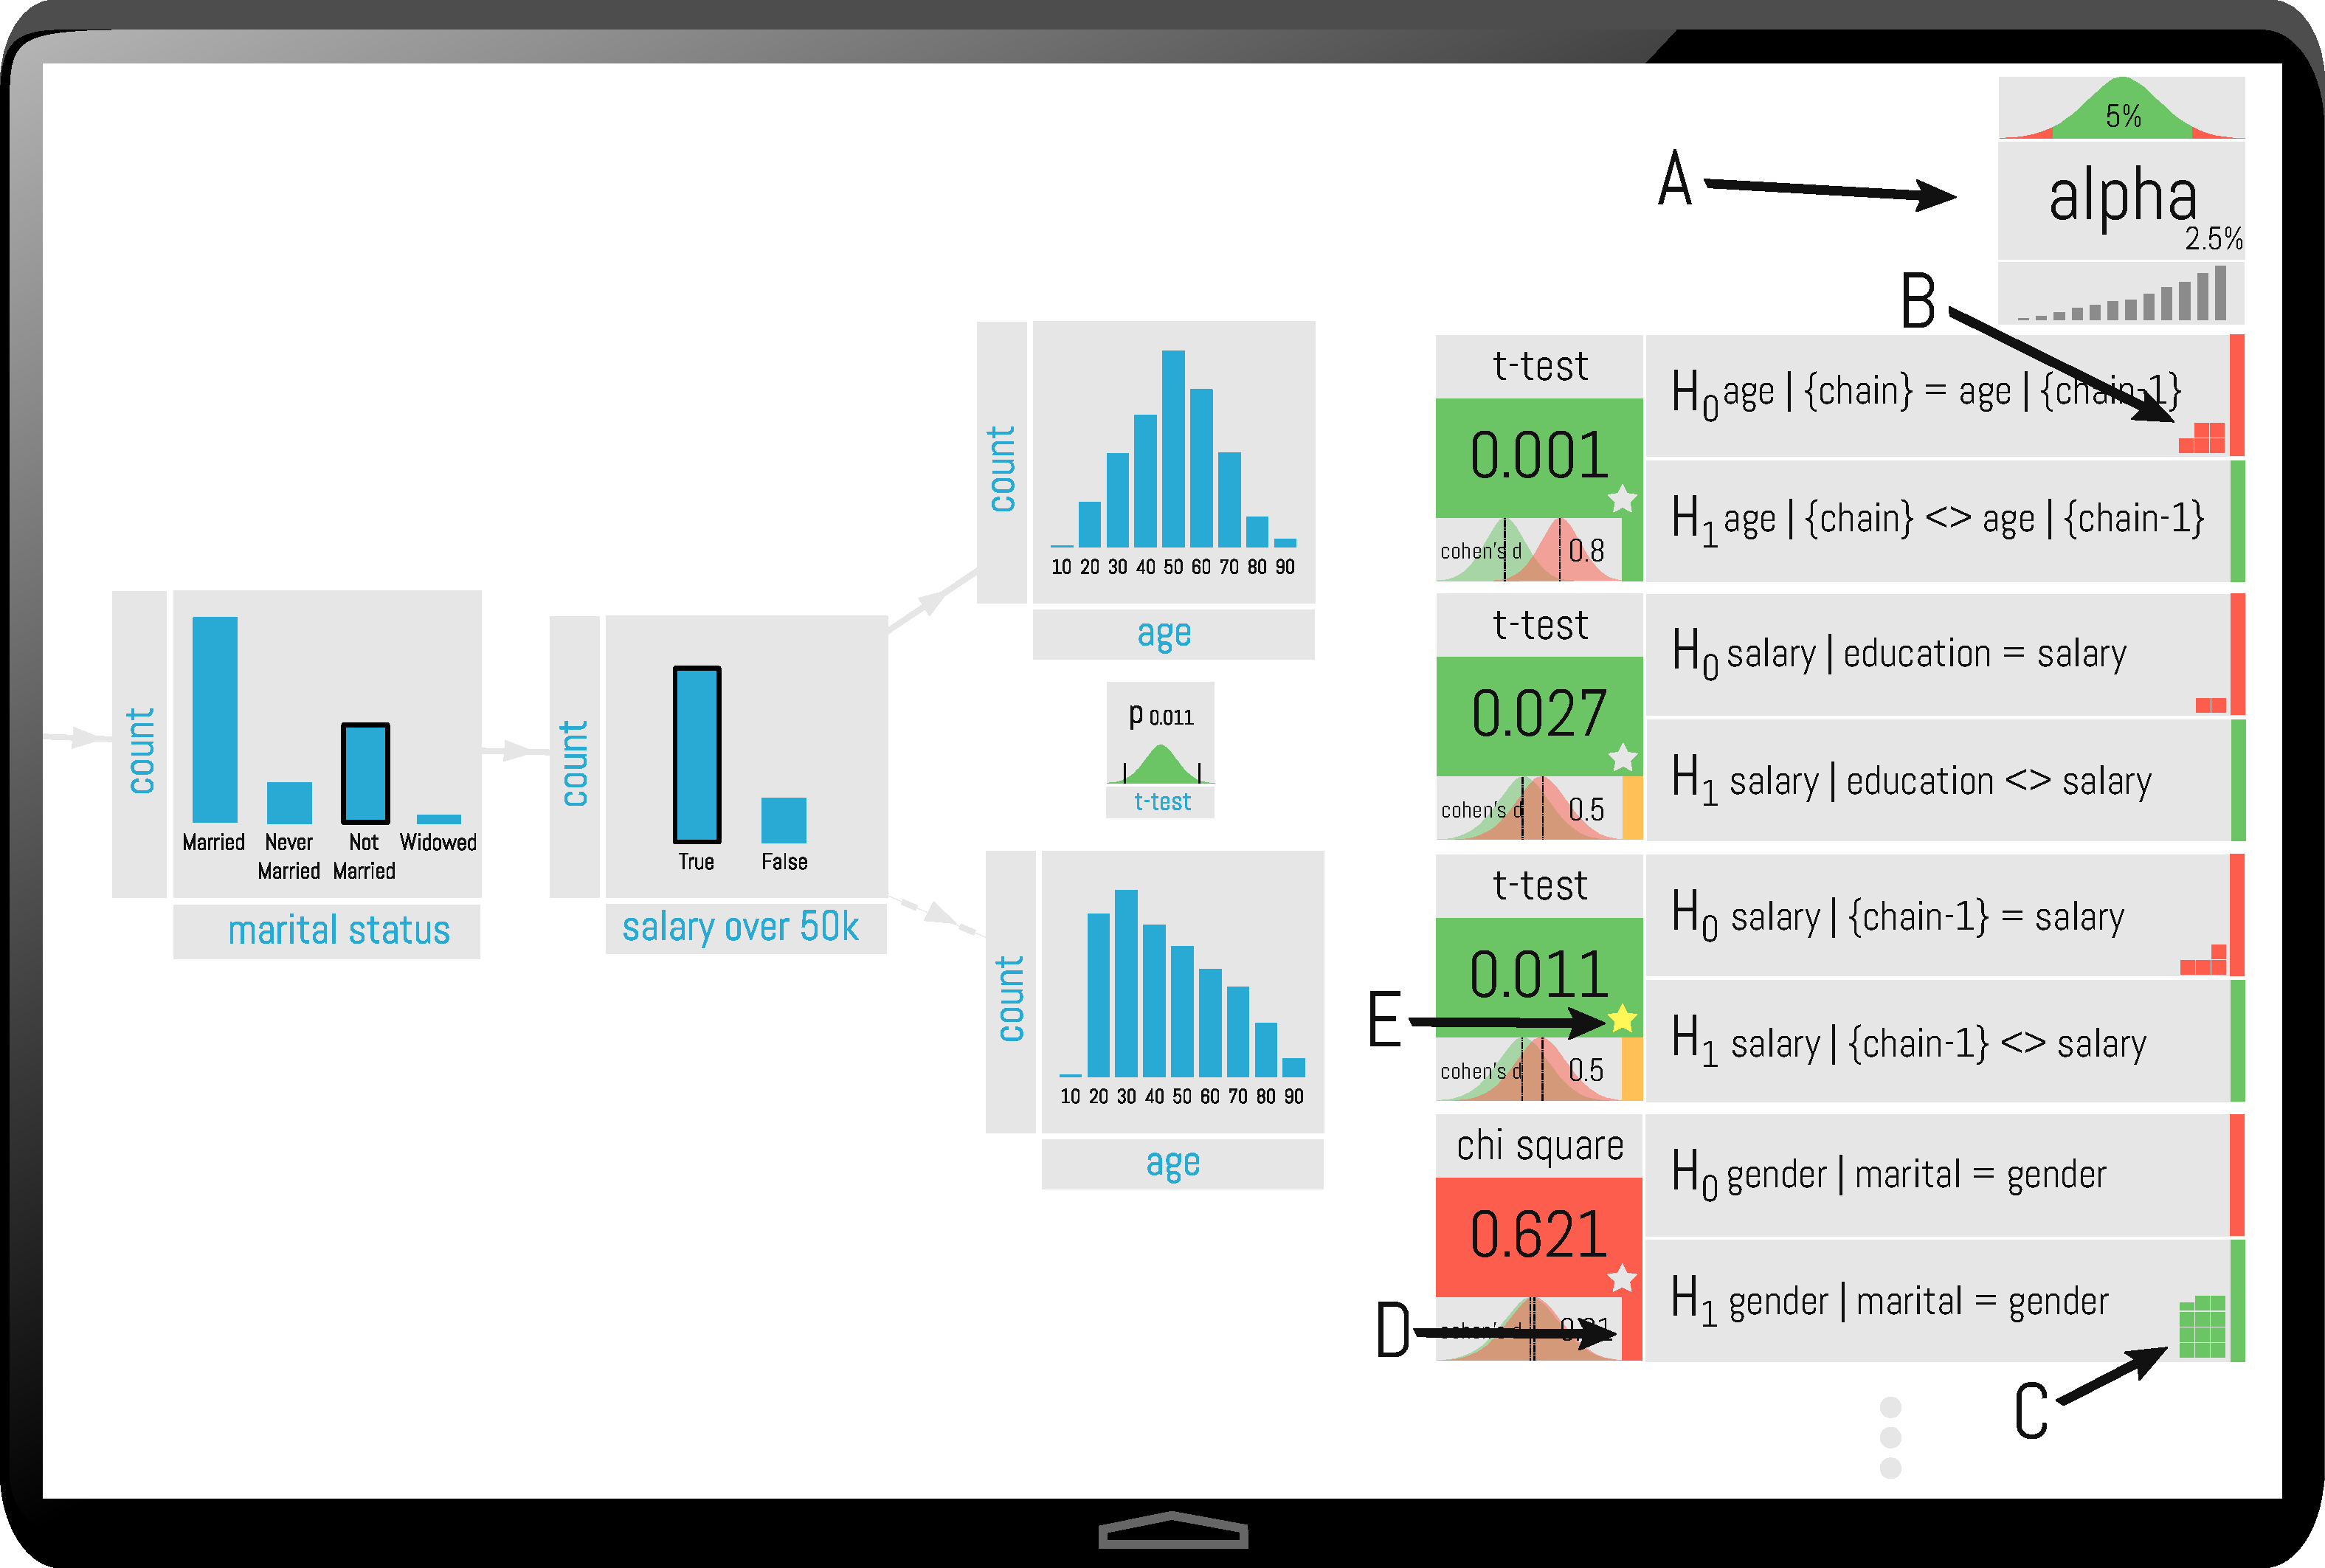
\includegraphics[width=0.48\textwidth]{figures/risk_controller}
\caption{The \system{} User Interface}
\label{fig:ui}	
\end{figure}

\sam{todo: how to let user specify hypotheses; remove (B); hypothesis re-test once data added; past hypothesis lookup/redraw}
The user interface of \system{} features an unbounded 2D canvas where visualizations can be laid out in a free form fashion (Figure~\ref{fig:ui}). A ``risk-gauge'' on the right-hand side of the display (Figure~\ref{fig:ui} (A)) serves two purposes: 
\begin{itemize}
    \item To give user a summary of the control procedure (e.g., the budget for the false discovery rate set to 5\% with current remaining wealth of 2.5\%;
    \item To provide access to a scrollable list of all the hypotheses that have been explored.
\end{itemize}
Each list entry displays details about an observation and its statistical significance.  The text labels describe the null and alternative hypotheses concerning each observation and the corresponding hypothesis tests and \pvals. Each color coded tile indicates whether the observation is statistically significant or insignificant, which corresponds to green or red respectively.  The distributions of null and alternative hypotheses and the color coded effect size are also visualized (D).  To help the user understand the effect of data collection, the sample size estimate for the current significance level is displayed for each hypothesis test assuming the effect size is fixed (C).  For example, the five green squares in (C) indicates approximately five times the current data size with the same effect size would make this observation significant. Finally, important observations can be marked by tapping the ``star'' icons (E).

\subsection{Backend}
\label{sec:backend}
\sam{todo: describe system design choices, such as how to generate null hypotheses given user interactions, how to progressively compute marginalized false discovery rate in parallel, etc.}

\section{Scenarios}
\label{sec:scenarios}



\section{Conclusion}
\label{sec:conclusion}
Visual data exploration and recommendation examines large number of observations, and if not correctly controlled, would mistake visually significant results as statistically significant.  Recent theoretical advance in multiple comparison problem and control procedures adds the desirable property of interactivity to data exploration~\cite{zhao2016controlling}.  \system{} implements these interactive procedures. The pen-and-touch userface interface provides a smooth user experience.  The \system{} backend combines functional reactive programming and progressive approximation to achieve practical interactivity and scalability.

%\section{Acknowledgments}
%This research is funded in part by the Intel Science and Technology Center for Big Data, the NSF CAREER Award IIS-1453171, the Air Force YIP AWARD FA9550-15-1-0144, NSF IIS-1514491, and gifts from SAP, Oracle, Google, Mellanox, and Amazon.

%\clearpage
\balance
\begin{scriptsize}
\bibliographystyle{abbrv}
\bibliography{bib}
\end{scriptsize}

\end{document}